\section{Active Optics System Commissioning}
\label{sec:aos_commissioning}

The goals for commissioning of the Active Optics System (AOS) with ComCam are to demonstrate that we can align the telescope optics, determine and correct for optical aberrations using the hexapods and bending modes for M2 and M1M3, and apply these corrections as a closed loop system. A stretch goal is to demonstrate that, for the limited field-of-view of ComCam, we can meet the image quality requirements of the LSST system (i.e., with the optical system delivering less than 0.4 arcseconds to the image quality budget) and do so consistently as a function of elevation and temperature. We have achieved many of these goals, but there are still significant challenges in delivering seeing limited images consistently as a function of variable observing conditions.

AOS commissioning started on 2024-10-24 with the first ComCam images delivering a 1.7 arcsecond full-width half-maximum (FWHM) image quality. This is a testament to the exceptional metrology work of the engineering and optical teams during assembly and to the optimization of the Look-Up Table (LUT) for all the active optics components using the  laser tracker data as well as mirror force balance data throughout 2024. 

Sub-arcsecond image quality was achieved on the night of 2024-11-06, with a best image quality of 0.65 arcsecond FWHM on the night of 2024-11-15. Corrections for the optical aberrations have been achieved using two independent approaches; the TIE wavefront estimation algorithm, which is an inversion method, and the Danish wavefront estimation algorithm, which is a forward modeling method. The AOS system was able to achieve closed-loop corrections across varying elevations and stellar densities, with most optical modes utilized (excluding the three highest-order modes on M2). Closed-loop operations have been run autonomously by the observing specialists to show that the scripts and procedures are mature. Preparations are underway to prototype a fully autonomous survey-mode triplet-taking block before the conclusion of ComCam's on-sky operations.

While we have demonstrated that Rubin can achieve the optical performance requirements for the AOS system there are significant challenges in meeting the optical performance requirements consistently as a function of temperature and elevation. It is not currently clear which aspects of the optical system are limiting its performance but the AOS team is working to understand the source of high levels of defocus and some amount of astigmatism that are present in the Zernike measurements. The team is also working to improve the computational efficiency of the system, which currently takes 5 minutes to complete a closed-loop iteration. 

After significant development, the AOS algorithms appear robust for a range of source densities and image qualities. A number of failure modes of the AOS software are present and being investigated. These include failures in processing images through Rapid Analysis when donuts cannot be detected on all sensors, and difficulty in measuring the wavefront when the images are significantly defocused (e.g., when the intra or extra focal images appear in focus). The AOS team is working to improve the robustness of the system to monitor these and other failure modes.

Figure~\ref{fig:aos} shows the FWHM delivered by the optical system (black line) as we correct the alignment and bending modes of the mirrors and camera over the nights 2024-11-25 to 2024-12-01. The FWHM is estimated from the Zernike amplitudes measured from out-of-focus donuts. The grey and blue lines are the 500nm and zenith corrected image qualities measured by SOAR and from the Rubin images respectively. The dashed green line is the 0.25 arcseconds image quality requirement for the telescope optics. From these measurements the AOS system is shown capable of meeting the image quality requirements. Delivering this consistently and without significant fine tuning is the current focus for the AOS team.

\begin{figure}
    \centering 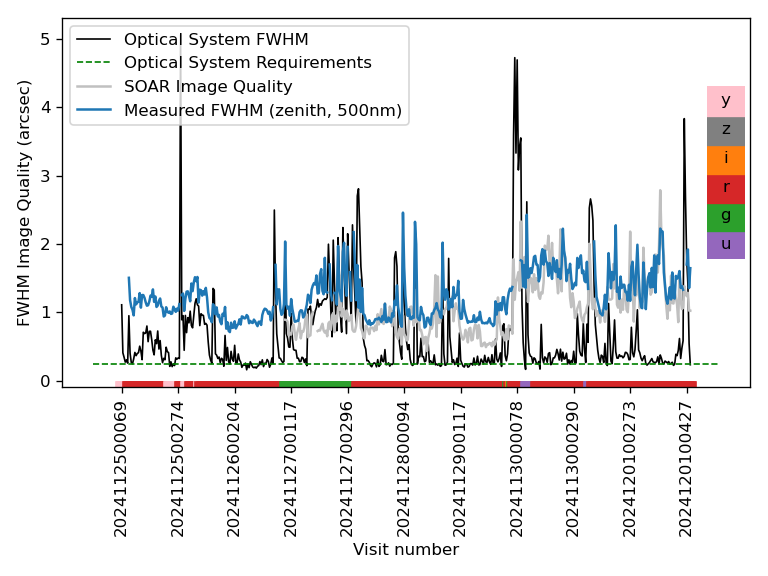
\includegraphics[width=0.7\textwidth]{figures/optical_performance.png}
    \caption{The FWHM delivered by Rubin (blue), the image quality from Rubin's optical system estimated from the AOS (black), and the image quality measured by SOAR (gray). The Rubin and SOAR measured FWHMs are corrected to 500nm and zenith.}
    \label{fig:aos}
\end{figure}

%z22 z11

\subsection{Initial Alignment}
Initial alignment of the AOS utilizes an updated laser tracker nominal frame based on a Final Element Analysis Model.  This ensures that the system is brought into focus prior to the start of observations.  Combined with a measurement of the impact of gravity on the telescope, these refinements simplified the alignment process, demonstrating the value of accurate laser tracker data. Once we were able to get on-sky images using curvature wavefront sensing, we finalized the initial state of the hexapods position to ensure a well aligned system at the start of the night. Work is ongoing to understand the stability of the initial hexapod and bending mode positions across nights to determine how well we can predict the configuration of the AOS system at the start of each night. 


\subsection{Coordinate Systems}
During the first few weeks, significant effort was devoted to understanding and refining coordinate systems at different steps of the active optics closed-loop process (wavefront sensor estimation and correction calculation). We conducted the test by introducing one degree of freedom at a time and correcting for it. We identified a rotation discrepancy in ComCam's installation compared to the expected design, requiring 
adjustments in our alignment procedures. The coordinate discrepancies were resolved empirically in the early AOS tests. Based on these data the expected as-delivered coordinate system(s) for the mirrors, hexapods, and sensors will need to be derived from first principles and validated prior to AOS observations with LSSTCam.


\subsection{Wavefront estimation}
The wavefront estimator proved robust across diverse observing conditions of seeing, mount elevation and a few filters (r,i and y band) 
On dense fields such as 47 Tuc or NGC 253, the estimator provided accurate results for all sensors except the central one.  Comparison of observed PSFs with simulations confirmed the accuracy of Rubin's ray-tracing software, \texttt{Batoid}.

Wavefront estimation and closed-loop convergence has been demonstrated using \texttt{TIE} and \texttt{Danish}. Other advancements include the implementation of sparse Zernikes, allowing selective inclusion of Zernike polynomial terms while minimizing cross-contamination 
of modes with identical azimuthal dependencies.

Despite delivering good optical quality, Zernike measurements indicate persistently high levels of defocus and some amount of astigmatism. We are continuing to investigate the source and impact of these measurements.

\subsection{Closed Loop}
Following resolution of initial issues with the AOS pipelines, closed-loop operations were achieved across varying elevations and filters (u, g, r, i, z, and y).  Most optical modes were utilized, excluding the three highest-order modes on M2.  Consistency in results across nights confirmed the need for further refinement of the LUT. In favorable seeing conditions, the system achieved sub-arcsecond image quality, with FWHM as low as 0.65 arcseconds. Autonomous closed-loop operations were run by observers, demonstrating the maturity of the system. 

%Zernike-based AOS FWHM  contributions confirmed the system's convergence to exceptional image quality. 

The closed loop process still takes 5min often requiring 5 or more iterations. The best performance for the closed loop achieved convergence in two iterations but delivering this consistently has not been achieved and tuning the closed-loop gain and making further adjustments to improve computational  efficiency remains a priority for the team.

\subsection{LUT}
The LUT underwent initial validation across elevations, azimuths, and rotator angles, 
leading to incremental improvements. While these updates enhanced performance, 
further refinements are needed to address second-order dependencies. Insights 
from ComCam data will inform these efforts, ensuring readiness for LSSTCam, which 
may present distinct challenges due to its larger focal plane and optical system.



\subsection{Lessons Learned and Next Steps}
\textbf{Lessons Learned}
- Coordinate Systems: Precision and methodical testing of coordinate systems are essential. 
Starting with foundational tests and incrementally increasing complexity ensures reliability.
- Observer Training: Comprehensive documentation, including a subsystem overview and closed-loop procedures, 
significantly enhances observer support capabilities.
- Closed-Loop Performance: Iterative testing and tuning of the closed-loop system are essential for delivering a consistently high image quality as a function of temperature, elevation, and other observing conditions. Achieving this performance consistently and without significant fine tuning will be a significant challenge.
- Engagement and Morale: Fun and engaging night summaries boost team morale, fostering a collaborative 
and motivated work environment.
- Transferability: Some ComCam lessons learned, particularly LUT and coordinate system adjustments, 
will not fully transfer to LSSTCam, requiring repeated validation.

\textbf{Next Steps}
- Conduct step-by-step closed-loop validations for LSSTCam, validating signs and rotations for intentional perturbations.
- Collaborate with the Camera Team to anticipate and mitigate known camera tilts.
- Implement and validate tests tailored to LSSTCam's larger focal plane dimensions.
- Prepare RubinTV and donutViz for full-array LSSTCam mode and automate its execution for all triplet-taking sequences.
- Adapt MTAOS to run as a continuous background task, supporting survey-mode operations.
- Optimize the AOS pipeline for speed, including binning and ISR performance improvements.


